\section{Results}
\label{sec:results}
In this section we'll look at the results we got from each of the different techniques outlined in \autoref{sec:methods}.

\paragraph{Execution notes.}
All the results were obtained by running our program with about 16 GB of working memory and 1 core per instance. The system running our program was equipped with an Intel Xeon \footnote{The cluster we worked on, is more thoroughly described here: \url{https://docs.dei.unipd.it/en/CLUSTER/Overview}}. The runtime for a sweep on the selected subsample rates is on the order of a few hours.

\subsection{Subsampling on the whole genome}
\begin{figure}[ht!]
    \centering
    \begin{subfigure}[t]{0.48\textwidth}
    \centering
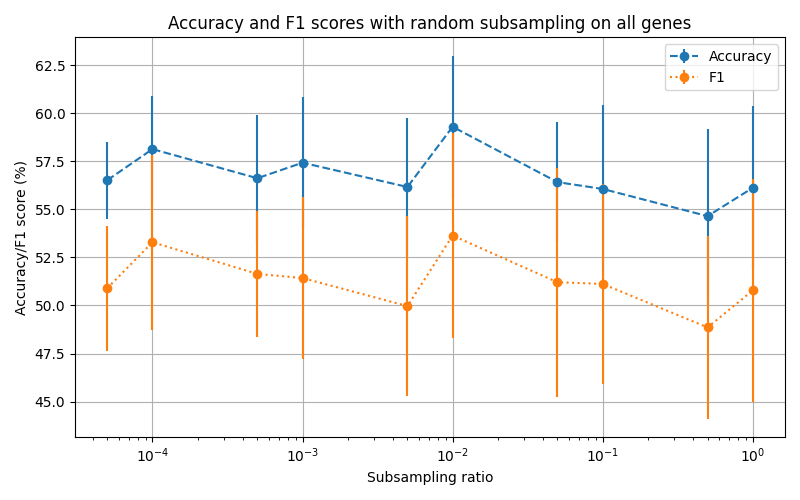
\includegraphics[width=\columnwidth]{figures/subsample_plot.png}
\caption{Plot of the accuracy and F1 scores when subsampling uniformly on the whole genome.}
\label{fig:res1a}
    \end{subfigure}
    \begin{subfigure}[t]{0.48\textwidth}
    \centering
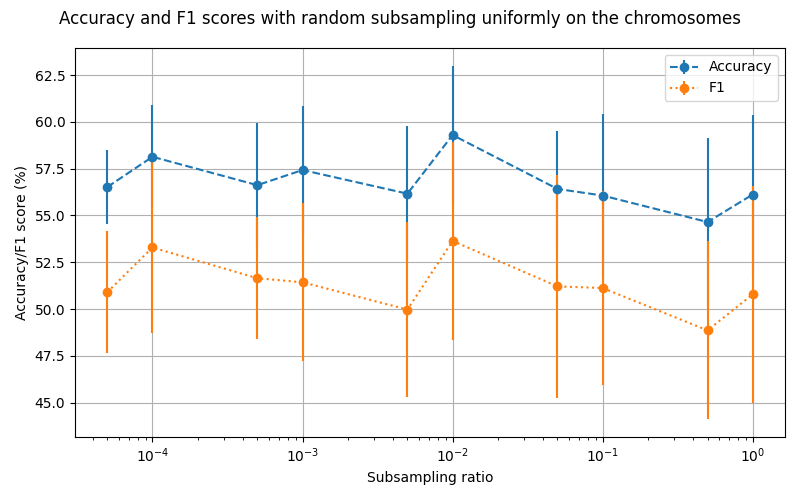
\includegraphics[width=\columnwidth]{figures/uniform_sample_low_ratio.png}
\caption{Plot of the accuracy and F1 scores when subsampling uniformly on each chromosome.}
\label{fig:res1b}
    \end{subfigure}
\caption{Plots of scores while subsampling the whole genome.}
\label{fig:res1}
\end{figure}

The first simple tests were done selecting a random subset of genes among all the SNPs that we had. The results for each subsampling rate are shown in \autoref{fig:res1}.
These plots show a mostly flat picture, both for the accuracy and F1 score there isn't a definite trend or variation as a function of the subsampling rate.

The only exception to this is \autoref{fig:res1a}, that shows a diminishing trend with the smallest subsampling rates. Nevertheless both of the last two data points are compatible with the middle points.

Note that the values at subsampling rate $1 = 10^0$ are the same in the two plots of \autoref{fig:res1]}. This single values could be slightly lower than the other values just because of random variation in the testing setup.

\subsection{Annotated genes subsampling}
\begin{figure}[ht]
    \begin{center}
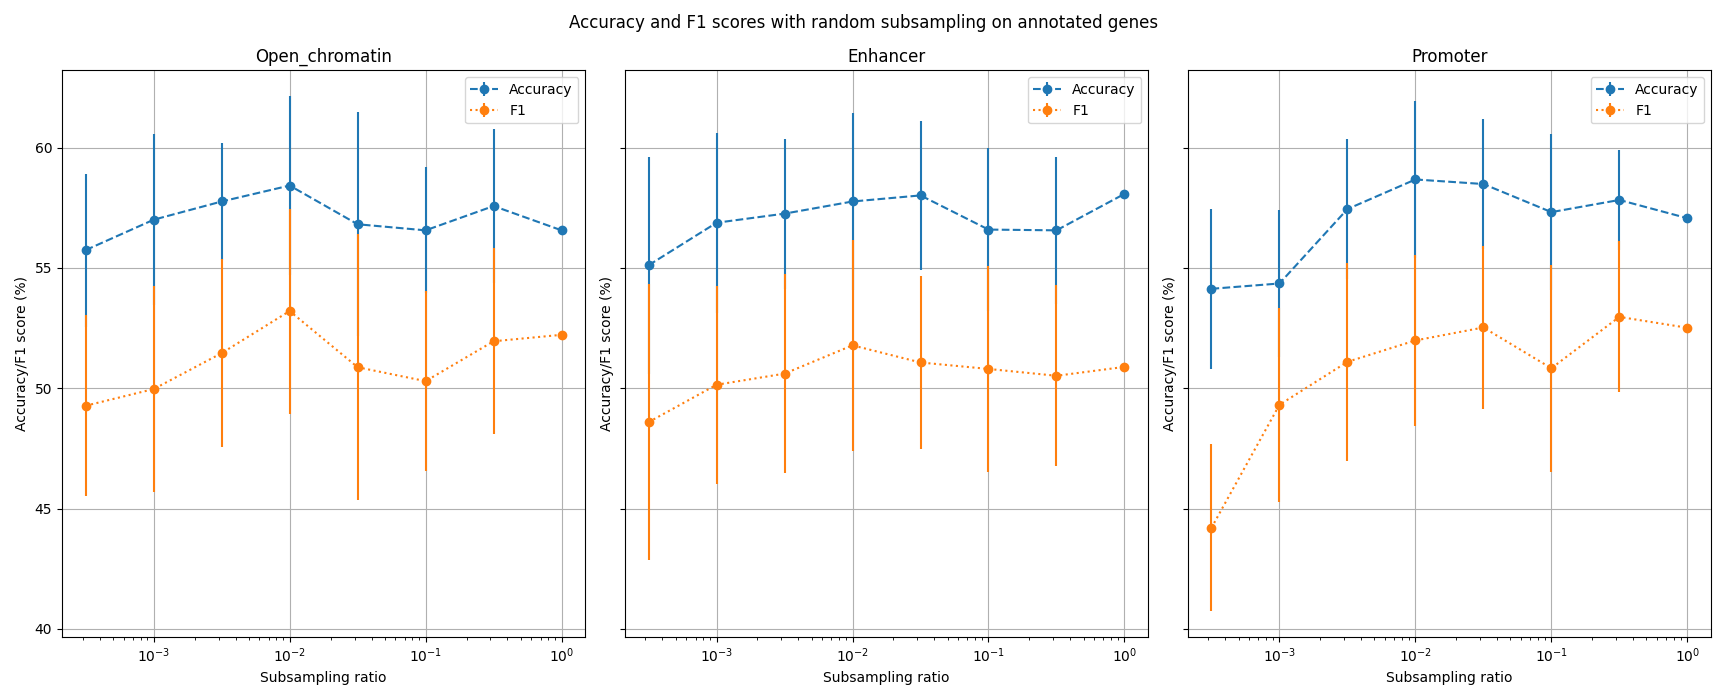
\includegraphics[width=\textwidth]{figures/subsample_annotated.png}
    \end{center}
\caption{Plots of the accuracy and F1 scores while using only genes with given tissue number, on the $x$-axis there is the subsampling rate.}
\label{fig:res3}
\end{figure}
\begin{figure}[ht]
    \begin{center}
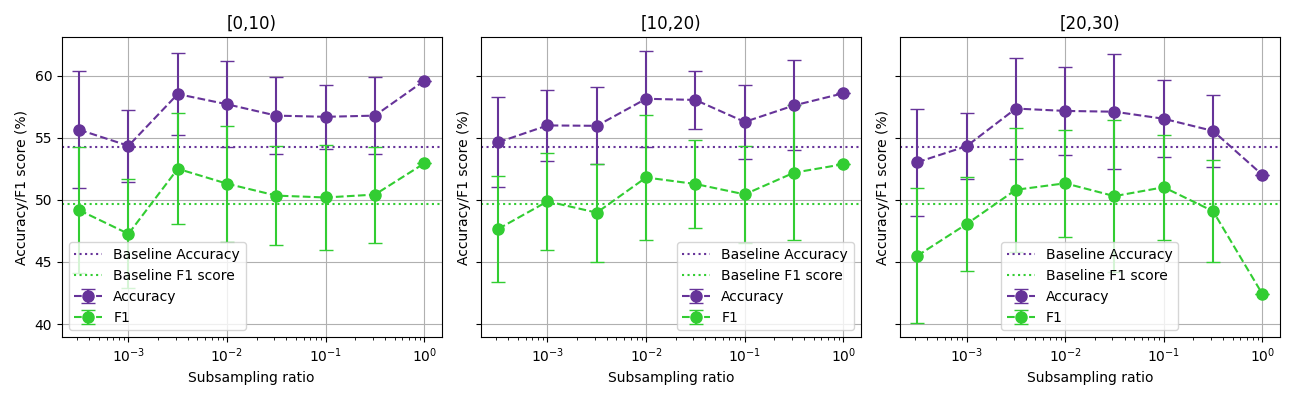
\includegraphics[width=\textwidth]{figures/subsample_ntissue.png}
    \end{center}
\caption{Plots of the accuracy and F1 scores while using only genes with given tissue number, on the $x$-axis there is the subsampling rate.}
\label{fig:res4}
\end{figure}

\subsection{Considerations on the results}
Our results suck a lot.
